






\subsection{Credit loss Distrihution CR-4}




\subsubsection{EL、UL、ULC（重要的不能再重要了）}

\renewcommand{\arraystretch}{2}

\begin{center}
    \adjustbox{max width=\textwidth}{
        \begin{tabular}{|p{0.8\textwidth}|p{0.4\textwidth}|}

    \hline
    \multicolumn{2}{|c|}{(1)预期损失 (Expected Loss， EL):指在未来一段时间(通常是一年)可能发生的平均损失。 也就是损失的期望值。} \\
    \cline{1-2}
    单个资产:\newline  \(\mathrm{{EL}}\left( \% \right)  = \mathrm{{PD}} * \mathrm{{LGD}}\) \newline   \(\mathrm{{EL}}\left( \$ \right)  = \mathrm{{PD}} * \mathrm{{LGD}} * \mathrm{{EAD}}\) 【主要用这个公式】 & \(\mathrm{{PD}} \rightarrow\) 信用评级、 \(\mathrm{{CS}}\) 、莫顿模型   \newline  计算 PD   \newline   LGD=loss rate=1-回收率 \newline   EAD， 也写作 exposure amount (EA) \\
    \cline{1-2}
    组合: \({\mathrm{{EL}}}_{\mathrm{P}} = \mathop{\sum }\limits_{{i = 1}}^{n}{\mathrm{{PD}}}_{\mathrm{i}} \times  {\mathrm{{LGD}}}_{\mathrm{i}} \times  {\mathrm{{EAD}}}_{\mathrm{i}}\) \newline 两资产组合:\({\mathrm{{EL}}}_{\mathrm{P}} = {\mathrm{{PD}}}_{1} \times  {\mathrm{{LGD}}}_{1} \times  {\mathrm{{EAD}}}_{1} + {\mathrm{{PD}}}_{2} \times  {\mathrm{{LGD}}}_{2} \times  {\mathrm{{EAD}}}_{2}\) & 和资产之间的相关性 \(\rho\) 无关 \\
    \cline{1-2}
    \multicolumn{2}{|p{1.2\textwidth}|}{(2)非预期损失 (Unexpected Loss， UL): \par  UL is the standard deviation of credit losses， that is， the standard deviation of actual credit losses around the expected loss average (EL). \par  切记: 在这个科目中， UL 的概念， 与一级以及二级其他科目中的 Unexpected Loss 概念不 同。} \\
    \cline{1-2}
    单个资产:\newline \(\mathrm{{UL}} = \mathrm{{EAD}} \times  \sqrt{{\mathrm{{PD}}}_{\mathrm{i}} \times  {\sigma }_{\mathrm{{LGD}}}^{2} + {\mathrm{{LGD}}}^{2} \times  {\sigma }_{\mathrm{{PD}}}^{2}}\) \newline Bernoulli 伯努利分布 \(\rightarrow  {\sigma }_{\mathrm{{PD}}}^{2} = \mathrm{{PD}} \times  \left( {1 - \mathrm{{PD}}}\right)\) & \({\sigma }_{\mathrm{{LGD}}}^{2} :\) LGD 的方差\newline \({\sigma }_{\mathrm{{PD}}}^{2} : \mathrm{{PD}}\) 的方差 \\
    \cline{1-2}
    组合: \({\mathrm{{UL}}}_{\mathrm{p}} = \mathop{\sum }\limits_{\mathrm{i}}\mathop{\sum }\limits_{\mathrm{j}}{\rho }_{\mathrm{i}，\mathrm{j}} \times  {\mathrm{{UL}}}_{\mathrm{i}} \times  {\mathrm{{UL}}}_{\mathrm{j}}\) 两资产组合: \({\mathrm{{UL}}}_{\mathrm{p}} = \sqrt{{\mathrm{{UL}}}_{1}^{2} + {\mathrm{{UL}}}_{2}^{2} + 2 \times  {\rho }_{1，2} \times  {\mathrm{{UL}}}_{1} \times  {\mathrm{{UL}}}_{2}}\) 若单个资产的 \(\mathrm{{UL}}\) 相等，相关系数相等 \(\rightarrow  {\mathrm{{UL}}}_{\mathrm{n}} = \mathrm{{UL}} \times\)  \(\sqrt{\mathrm{n} + \mathrm{n} \times  \left( {\mathrm{n} - 1}\right)  \times  \mathrm{\rho }}\) & \({\rho }_{\mathrm{i}，\mathrm{j}}\) : 资产 \(\mathrm{i}\) 和 \(\mathrm{j}\) 的违约相关性 \\
    \cline{1-2}
    \multicolumn{2}{|p{1.2\textwidth}|}{(3) Unexpected Loss Contribution (ULC):\newline ULC 是指单个资产 (如 loan) 对整个 UL 的边际贡献。即衡量一个特定资产在整个组合可能 出现的损失中占了多大的份额。【重点掌握两资产】} \\
    \cline{1-2}
    \({\mathrm{{ULC}}}_{\mathrm{i}} = \frac{{\mathrm{{UL}}}_{\mathrm{i}} \times  \mathop{\sum }\limits_{\mathrm{j}}{\rho }_{\mathrm{i}，\mathrm{j}} \times  {\mathrm{{UL}}}_{\mathrm{j}}}{{\mathrm{{UL}}}_{\mathrm{p}}}\) & \phantom{X} \\
    \cline{1-2}
    \multicolumn{2}{|p{1.2\textwidth}|}{两资产:\newline \({\mathrm{{ULC}}}_{1} = \frac{{\mathrm{{UL}}}_{1}^{2} + {\rho }_{\mathrm{i}，\mathrm{j}} \times  {\mathrm{{UL}}}_{1} \times  {\mathrm{{UL}}}_{2}}{{\mathrm{{UL}}}_{\mathrm{p}}}  \);     
    \({\mathrm{{ULC}}}_{2} = \frac{{\mathrm{{UL}}}_{2}^{2} + {\rho }_{\mathrm{i}，\mathrm{j}} \times  {\mathrm{{UL}}}_{1} \times  {\mathrm{{UL}}}_{2}}{{\mathrm{{UL}}}_{\mathrm{p}}}\) ； \({\mathrm{{ULC}}}_{1} + {\mathrm{{ULC}}}_{2} = {\mathrm{{UL}}}_{\mathrm{p}}\)} \\
    \cline{1-2}
    前提: \(\mathrm{n}\) 笔 loan; 每笔 loan 规模相同、风险特质相同\newline \({\mathrm{{ULC}}}_{\mathrm{i}} = \frac{{\mathrm{{UL}}}_{\mathrm{p}}}{\mathrm{n}} = {\mathrm{{UL}}}_{\mathrm{i}} \times  \sqrt{\frac{1}{\mathrm{n}} + \rho  \times  \left( {1 - \frac{1}{\mathrm{n}}}\right) }\) \newline 前提: \(\mathrm{n}\) 比较大时  \newline \({\mathrm{{ULC}}}_{\mathrm{i}} = {\mathrm{{UL}}}_{\mathrm{i}} \times  \sqrt{\rho }\) & the correlation between assets increases， the bank suffers from concentration risk 集中度风险。 \\
    \cline{1-2}
    \hline
    \end{tabular}
    }
    \end{center}



\begin{comment}

\renewcommand{\arraystretch}{1.2}




\begin{tabular}{|p{0.25\textwidth}|p{0.7\textwidth}|}
\hline
\multicolumn{2}{|l|}{\textbf{(1) 预期损失 (Expected Loss， EL):}} \\
\hline
定义 & 指在未来一段时间（通常是一年）可能发生的平均损失，也就是损失的期望值。\\
\hline
单个资产 & \( EL(\%) = PD \times LGD \)\\
         & \( EL(\$) = PD \times LGD \times EAD \quad \text{【主要用这个公式】} \)\\
\hline
术语定义 & 
\begin{itemize}
  \item PD = 信用评级、CS、莫顿模型计算PD
  \item LGD = loss rate = 1 - 回收率
  \item EAD = 暴露金额（Exposure Amount， EA）
\end{itemize} \\
\hline
组合 & \( EL_p = \sum_{i=1}^n PD_i \times LGD_i \times EAD_i \)\\
\hline
两资产组合 & \( EL_p = PD_1 \times LGD_1 \times EAD_1 + PD_2 \times LGD_2 \times EAD_2 \) \\
\hline
\multicolumn{2}{|l|}{\textbf{(2) 非预期损失 (Unexpected Loss， UL):}} \\
\hline
定义 & UL 是实际损失围绕预期损失的标准差 \\
\hline
单个资产 & \( UL = EAD \times \sqrt{PD_i \times \sigma^2_{LGD} + LGD^2 \times \sigma^2_{PD}} \) \\
\hline
注释 & \(\sigma^2_{LGD}\)：LGD 的方差；\(\sigma^2_{PD}\)：PD 的方差\\
     & Bernoulli伯努利分布：\(\sigma^2_{PD} = PD \times (1 - PD)\) \\
\hline
组合 & \( UL_p = \sum_i \sum_j \rho_{ij} \times UL_i \times UL_j \) \\
\hline
两资产组合 & \( UL_p = \sqrt{UL_1^2 + UL_2^2 + 2 \times \rho_{12} \times UL_1 \times UL_2} \) \\
\hline
等相关 & \( UL_p = UL \times \sqrt{n + n(n-1)\rho} \) \\
\hline
\multicolumn{2}{|l|}{\textbf{(3) Unexpected Loss Contribution (ULC):}} \\
\hline
定义 & ULC 是单个资产对整体 UL 的边际贡献，衡量其在组合中可能出现的损失中占了多少份额。\\
\hline
公式 & \( ULC_i = \frac{UL_i \times \sum_j \rho_{ij} \times UL_j}{UL_p} \) \\
\hline
两资产 & 
\( ULC_1 = \frac{UL_1^2 + \rho_{ij} \times UL_1 \times UL_2}{UL_p} \)\\
        & 
\( ULC_2 = \frac{UL_2^2 + \rho_{ij} \times UL_1 \times UL_2}{UL_p} \)\\
        & 
\( ULC_1 + ULC_2 = UL_p \)\\
\hline
n 笔 loan（规模相同） & 
\( ULC_i = \frac{UL_i}{UL_p} = \frac{1}{n} + \rho \times \left(1 - \frac{1}{n} \right) \)\\
\hline
结论 & 
the correlation between assets increases， the bank suffers from concentration risk 集中度风险。\\
\hline
\end{tabular}
\end{comment}







\subsubsection{Credit loss distribution and capital}

\begin{center}
    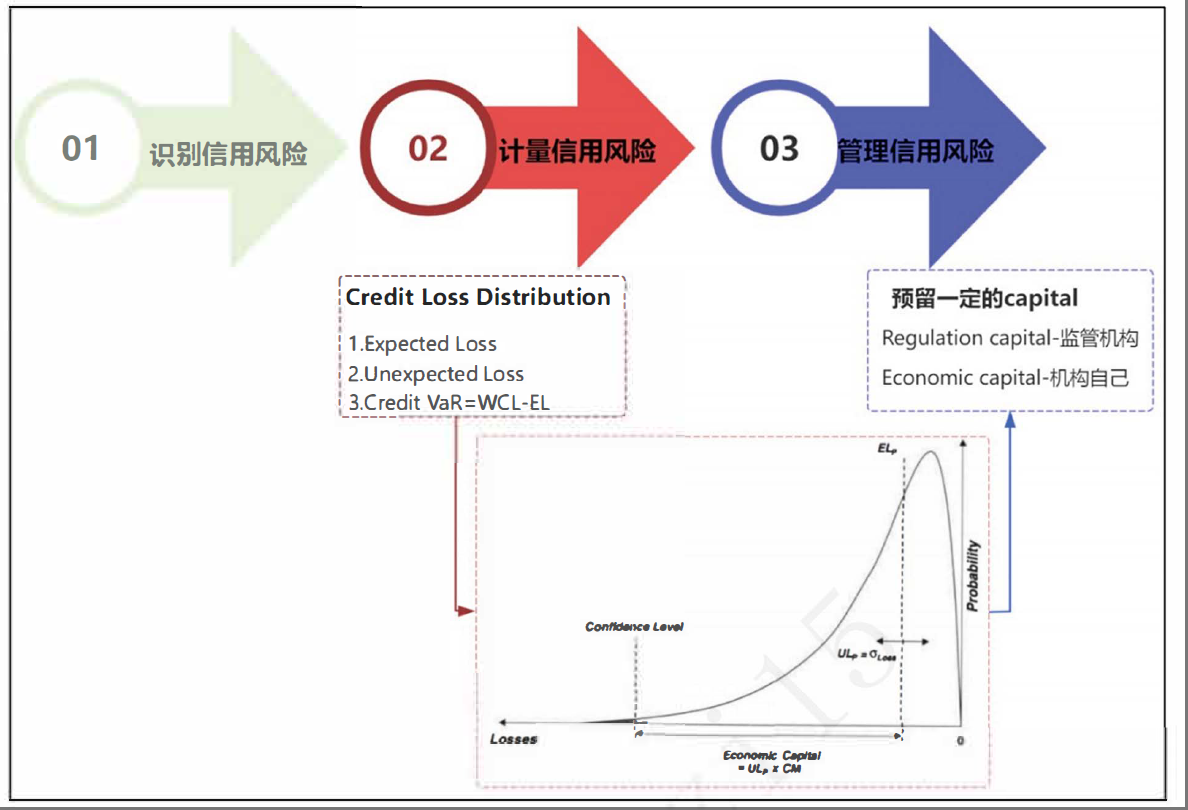
\includegraphics[width=1\textwidth]{images/creditvar.png}
    \end{center}
    \hspace*{3em} 

    \begin{itemize}
    \item  Capital multiplier(资本乘数， CM) is dependent on the overall credit quality
    of the portfolio and the confidence level.

    \begin{itemize}
       
   
        \item  信用质量变差， CM变大
        \item confidence level置信水平上升， CM变大
\end{itemize}
\end{itemize}









\begin{itemize}
    \item Credit Loss Distribution信用损失分布是一个概率分布， 描述在给定的时间
    段内（通常为一年）可能的信用损失及其发生的概率。
    \begin{itemize}

    \item  信贷风险不是正态分布的，而是高度倾斜(highly skewed)的，因为上升潜力仅限于最多收到承诺的付款，在极少数情况下会损失大量资金。 【收益有限，
    比如利息；损失比较大， 比如本金】
    \item  信用损失的期望一预期损失(Expected Loss， EL)
    \item  信用损失的标准差一非预期损失(Unexpected Loss， UL)
\end{itemize}

    \item 可以用beta distribution建模信用风险损失．【关于beta 分布，无需了解太深】
    \begin{itemize}
        \item  尾部拟合工作的最佳方法是将分析（贝塔分布）解决方案与蒙特卡罗模拟等数值程序相结合。The tail-fitting exercise is best accomplished by combining the analytical (beta distribution) solution with a numerical
        procedure such as a Monte Carlo simulation.
        \item   在选定的置信水平下，利用贝塔函数的倒数，我们可以确定 CM，即资本乘数。Taking the inverse of the beta function at the chosen confidence level, we can determine CM, the capital multiplier. 给定置信水平， 拟合完分布， 倒求出资本乘数

    \end{itemize}

\end{itemize}


\subsubsection{Problems with the Quantification of Credit Risk}
\begin{itemize}
    \item 只考虑违约， 没考虑价值变化This approach assumes that
credits are illiquid assets.
\item  More liquid asset: a value approach would be more
suitable.
\item  借款人信用质量会变Multi-period nature of credits: the
expected and unexpected changes in the credit quality of the
borrowers (and their correlations).
\item  只考虑信用风险All other risk components (such as market
\item  and operational risk) are separated.
\end{itemize}




\subsection{Credit Value at Risk CR-10}


\subsubsection{Vasicek model
}

\begin{itemize}
\item 只考虑违约情况， 不考虑评级下调情况
\end{itemize}

\begin{itemize}
\item Vasicek's Gaussian copula model is a way of calculating high percentiles of the distribution of the default rate for a portfolio of loans.
\end{itemize}

\begin{itemize}
\item WCDR(T， X): the Xth percentile of the default rate distribution during a period of length \(\mathrm{T}\) .
\end{itemize}

\begin{itemize}
\item 也叫 worst case default rate 最差情况违约概率

 参数: probability of default in time T; PD; credit correlation(ρ)

\item 模型的目标:找到一个糟糕市场情况下的条件概率

\item The Basel Committee sets \(\mathrm{X} = {99.9}\) or regulatory capital in the internal ratings-based approach(IRB， 内部评级法).

\item Capital requirement(Credit VaR)=(WCDR- PD) × EAD × LGD

\[
\operatorname{WCDR}\left( {T,X}\right)  = N\left( \frac{{N}^{-1}\left( {PD}\right)  - \sqrt{\rho }{N}^{-1}\left( X\right) }{\sqrt{1 - \rho }}\right) N\left( \frac{{N}^{-1}\left( {PD}\right)  - \sqrt{\rho }{N}^{-1}\left( {0.001}\right) }{\sqrt{1 - \rho }}\right)
\]

 WCDR * LGD * EAD is the loss at this 99.9 percentile point.

 PD * LGD * EAD is the expected loss.

\begin{itemize}
\item For a large portfolio with \(n\) small loans， the \(X\) th percentile of the loss distribution can be approximated as:
\end{itemize}

组合: \(\mathrm{n}\) 笔贷款，每笔贷款只是组合的一小部分

\[
\mathop{\sum }\limits_{{i = 1}}^{n}{\mathrm{{WCDR}}}_{\mathrm{i}}\left( {\mathrm{T},\mathrm{X}}\right)  \times  {\mathrm{{EAD}}}_{\mathrm{i}} \times  {\mathrm{{LGD}}}_{\mathrm{i}}
\]

\item 巴塞尔协议二【在操作风险这个科目会进行更详细的介绍】

 IRB 基础法:银行自行估计:PD；巴塞尔规定:EAD、LGD 和 MA

 IRB 高级法:全部由银行自行估计

 但 \(\rho\) 均由巴塞尔规定给出

\end{itemize}



\begin{center}
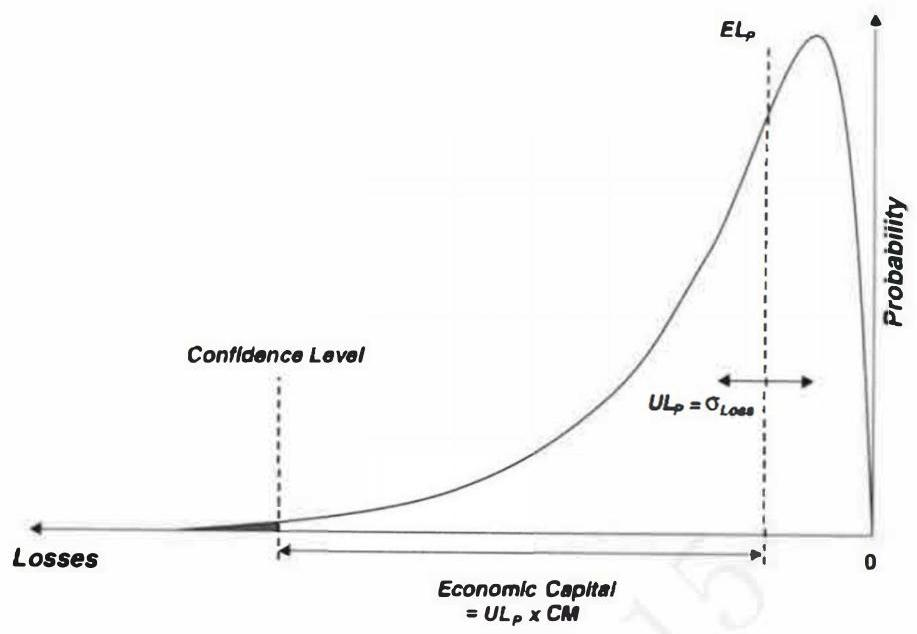
\includegraphics[width=0.7\textwidth]{images/0196660e-d86d-7ef6-8951-a48e2a482302_4_368_319_917_634_0.jpg}
\end{center}
\hspace*{3em} 

\subsubsection{CreditMetrics Model}

\begin{itemize}
\item 由 JPMorgan 于 1997 年提出
\end{itemize}

\begin{itemize}
\item 考虑了降级和违约的情况 (不仅仅只是违约情况)， 通过使用评级转换矩阵 rating transition matrix 进行蒙特卡罗模拟， 最终计算出跨所有对手方 (相关性)的 Credit Loss Distribution 信用损失分布 \(\rightarrow\) VaR。
\end{itemize}

\begin{itemize}
\item 评级可以是银行的内部评级或评级机构提供的评级。
\end{itemize}

\begin{itemize}
\item One-Year Ratings Transition Matrix
\end{itemize}

\begin{center}
\adjustbox{max width=\textwidth}{
\begin{tabular}{|c|c|c|c|c|c|c|c|c|}
\hline
\multirow{2}{*}{Initial Rating} & \multicolumn{8}{|c|}{Rating at Year-end} \\
\cline{2-9}
 & AAA & AA & A & BBB & BB & B & CCC/C & D \\
\cline{1-9}
AAA & 89.85 & 9.35 & 0.55 & 0.05 & 0.11 & 0.03 & 0.05 & 0.00 \\
\cline{1-9}
AA & 0.50 & 90.76 & 8.08 & 0.49 & 0.05 & 0.06 & 0.02 & 0.02 \\
\cline{1-9}
A & 0.03 & 1.67 & 92.61 & 5.23 & 0.27 & 0.12 & 0.02 & 0.05 \\
\cline{1-9}
BBB & 0.00 & 0.10 & 3.45 & 91.93 & 3.78 & 0.46 & 0.11 & 0.17 \\
\cline{1-9}
BB & 0.01 & 0.03 & 0.12 & 5.03 & 86.00 & 7.51 & 0.61 & 0.70 \\
\cline{1-9}
B & 0.00 & 0.02 & 0.08 & 0.17 & 5.18 & 85.09 & 5.66 & 3.81 \\
\cline{1-9}
CCC/C & 0.00 & 0.00 & 0.12 & 0.20 & 0.65 & 14.72 & 50.90 & 33.42 \\
\cline{1-9}
D & 0.00 & 0.00 & 0.00 & 0.00 & 0.00 & 0.00 & 0.00 & 100.00 \\
\cline{1-9}
\hline
\end{tabular}
}
\end{center}

\begin{itemize}
\item 使用 CreditMetrics 计算 Credit VaR

蒙特卡罗模拟:结合评级转移矩阵；每次模拟试验中，确定下一期信用评级。 \(\rightarrow\) 得出评级及对应概率

 计算信用风险时，需要考虑不同信用评级类别的信用利差期限结构 the term structure of credit spreads \(\rightarrow\) 结合无风险利率，得出折现率

可以直接使用现有市场数据代表信用利差， 或者使用综合指数预测的信用利差。

当考虑多个交易对手，可以通过高斯 copula 模型来建模违约相关性

\item 原版书例题: 【说明，在这个例题中，通过蒙特卡罗模拟已得出下一期的评级变化; 关于信用利差的期限结构也已经给出; 只有一个债券， 无需考虑相关性。最后得出 \(\rightarrow\) 信用损失分布】

\item Consider a company that owns a single two-year zero-coupon bond with a principal of \$1，000.

\(\diamond\) bond’s current rating is \(\mathrm{{BB}}\)

\textbackslash  ) the risk-free rate is 3\%

 the current credit spread is 200 basis points

 Rates are expressed with annual compounding.

The current price of the bond is \(1，{000}/\left( {{1.05}{}^{ \land  }2}\right)  = \$ {907.03}\) .

\item during the next month there is

* a 0.6\% chance that it will increase to BBB，

* a 98.5\% chance that it will stay the same，

* a 0.8\% chance that it will decrease to B， and

a 0.1\% chance that it will default. If it defaults， the bond will be worth \$400.

对于每个可能的评级类别， 有三个等可能的信用利差 credit spreads 分别为:

* B: 400bps、450bps、500bps

* BB: 160bps、200bps、240bps

* BBB: 80 bps、100bps、120bps

 分析:时间变化为 \({23}/{12} = {1.917}\) 年

 Default: 概率 \({0.1}\% ,\operatorname{loss} = {907.03} - {400} = {507.03}\)

 B 评级: \({500}\mathrm{{bps}}\) 情况，概率 \({0.8}\% /3 = {0.267}\%\) ，
 
 债券价值\(= {1000}/\left( {{1.08}^{ \land  }{1.917}}\right)  = {862.85},\;\) loss \(= {907.03} - {862.85} = {44.17}\)

 同理可得下表，显示了所有可能的结果及其概率 \(\rightarrow\) 信用风险损失分布

\begin{center}
\adjustbox{max width=\textwidth}{
\begin{tabular}{|c|c|c|c|c|}
\hline
Rating & Spread (bp) & Probability & Bond Value (\$) & Loss (\$) \\
\cline{1-5}
Default & \phantom{X} & 0.100\% & 400.00 & 507.03 \\
\cline{1-5}
B & 500 & 0.267\% & 862.85 & 44.17 \\
\cline{1-5}
B & 450 & 0.267\% & 870.56 & 36.47 \\
\cline{1-5}
B & 400 & 0.267\% & 878.38 & 28.65 \\
\cline{1-5}
BB & 240 & 32.833\% & 904.11 & 2.92 \\
\cline{1-5}
BB & 200 & 32.833\% & 910.72 & -3.70 \\
\cline{1-5}
BB & 160 & 32.833\% & 917.41 & -10.38 \\
\cline{1-5}
BBB & 120 & 0.200\% & 924.17 & -17.14 \\
\cline{1-5}
BBB & 100 & 0.200\% & 927.58 & -20.55 \\
\cline{1-5}
BBB & 80 & 0.200\% & 931.01 & -23.98 \\
\cline{1-5}
\hline
\end{tabular}
}
\end{center}

表中显示，如果置信水平高于 99.9\%， VaR 为 507.03 美元；

 如果置信水平在 99.9\%到 99.633\%之间， VaR 为 44.17 美元；以此类推。 当置信水平为 99\%时， VaR 为 2.92 美元。

\end{itemize}

\subsubsection{Credit Risk Plus (CreditRisk+)}

\begin{itemize}
\item Credit Risk Plus : 瑞士信贷金融产品(Credit Suisse Financial Products)在 1997 年提出
\end{itemize}

\begin{itemize}
\item 预测与保险公司的违约模型类似
\end{itemize}

\begin{itemize}
\item 只考虑违约情况， 不考虑评级下调情况
\end{itemize}

\begin{itemize}
\item 模型假设: 不同贷款或债务的违约事件是独立发生的。
\end{itemize}

\begin{itemize}
\item CreditRisk+模型中使用多种分布:
\end{itemize}

(1)二项分布 Binomial Distribution 和泊松分布 Poisson Distribution 【一级数量分析内容】

对于每笔贷款，假设其在一定时间内违约的概率为 \(\mathrm{q}\) ，利用二项分布 Binomial Distribution 可以估算出在给定的 \(\mathrm{n}\) 笔贷款中违约的数量 \(\mathrm{m}\) 。

\[
P\left( {X = m}\right)  = {C}_{n}^{m}{q}^{m}{\left( 1 - q\right) }^{n - m}
\]

\(\Leftrightarrow  \mathrm{E}\left( \mathrm{X}\right)  = \mathrm{{nq}}\)

\(\Leftrightarrow  \operatorname{Var}\left( \mathrm{X}\right)  = \mathrm{{np}}\left( {1 - \mathrm{q}}\right)\)

当贷款数目 \(\mathrm{n}\) 很大且每笔贷款的违约概率 \(\mathrm{q}\) 很小时，二项分布的概率分布形状会趋向于泊松分布，泊松分布更加简单且方便计算。 \(\left( {\lambda  = \mathrm{{nq}}}\right)\)

\[
P\left( {X = m}\right)  = \frac{{\left( nq\right) }^{m}{e}^{-{nq}}}{m!}
\]

(2)伽马分布 gamma Distribution 和负二项分布 negative binomial distribution: - the default rate(q)不确定， default rates vary greatly from year to year.

 假设 the expected number of defaults(qn)，服从伽马分布 gamma Distribution(mean \(\mu\) and standard deviation \(\sigma\) )，那么 The Poisson distribution then becomes a negative binomial distribution(负二项分布)

\[
\operatorname{Prob}\left( {m\text{ defaults }}\right)  = {p}^{m}{\left( 1 - p\right) }^{\alpha }\frac{\Gamma \left( {m + \alpha }\right) }{\Gamma \left( {m + 1}\right) \Gamma \left( \alpha \right) }
\]

【公式不要求掌握， 主要看里面的参数， 及对应的性质】 

\(\sigma\) [4] the negative binomial distribution = Poisson distribution.

 \(\sigma\) (1the likelihood of experiencing a large number of defaults increases. 拓展-gamma 分布图形:

\begin{center}
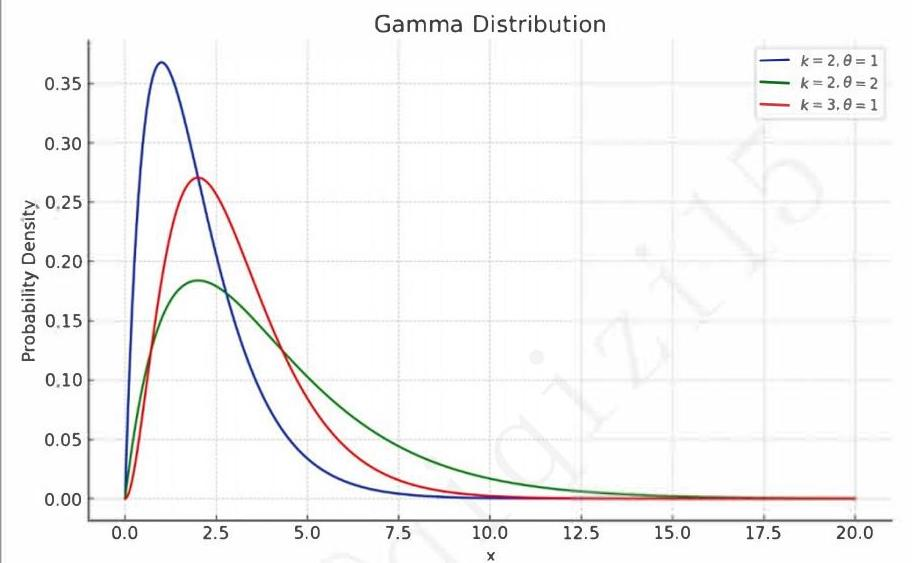
\includegraphics[width=0.7\textwidth]{images/0196660e-d86d-7ef6-8951-a48e2a482302_7_309_725_912_563_0.jpg}
\end{center}
\hspace*{3em} 

负二项分布图形:

\begin{center}
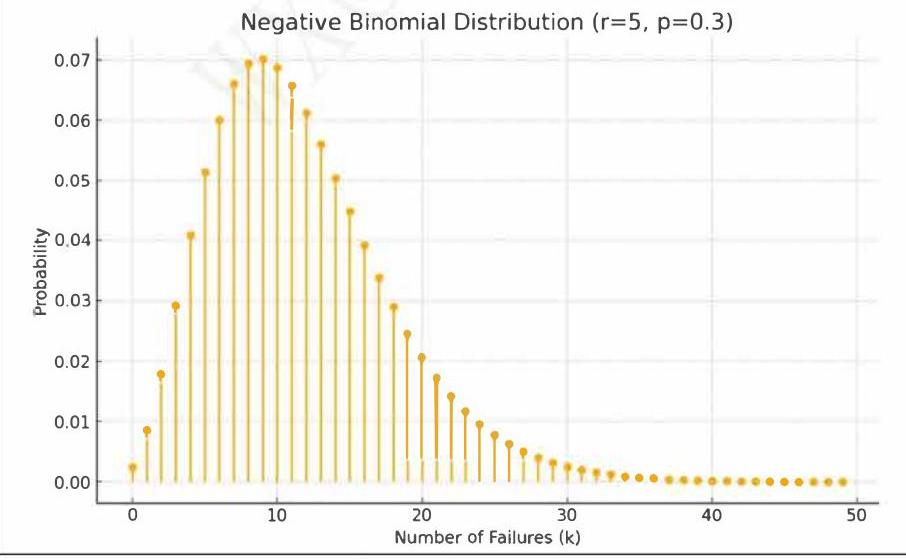
\includegraphics[width=0.7\textwidth]{images/0196660e-d86d-7ef6-8951-a48e2a482302_7_312_1349_906_560_0.jpg}
\end{center}
\hspace*{3em} 




\subsection{Default Correlation and Credit VaR CR-11-12}


\subsubsection{Default correlation违约相关性}


\begin{itemize}
    \item 衡量多个实体同时违约的趋势 Measures the tendency of multiple entities to default simultaneously
    
    \item 一家公司的违约可能引发另一家公司的违约，这被称为信用传染效应 (credit contagion effect)。
    
    \item 联合违约概率 joint default probability \(\left( {\pi }_{12}\right)\) : 在时间范围 \(\mathrm{T}\) 内两者都违约的概率
    
    \[
    \rho  = \frac{\operatorname{Cov}\left( {{X}_{1}{X}_{2}}\right) }{{\sigma }_{{X}_{1}}{\sigma }_{{X}_{2}}} = \frac{{\pi }_{12} - {\pi }_{1}{\pi }_{2}}{\sqrt{{\pi }_{1}\left( {1 - {\pi }_{1}}\right) }\sqrt{{\pi }_{2}\left( {1 - {\pi }_{2}}\right) }}
    \]
    
     \({\pi }_{1}\) : 资产 1 的违约概率
    
    \({\pi }_{2}\) : 资产 2 的违约概率
    
    拓展推导过程:
    
    一级数量科目，相关系数 \(\rho  = \frac{\operatorname{Cov}\left( {{\mathrm{X}}_{1}{\mathrm{X}}_{2}}\right) }{{\sigma }_{{\mathrm{X}}_{1}}{\sigma }_{{\mathrm{X}}_{2}}}\)
    
    \(\mathrm{E}\left( {\mathrm{X}}_{\mathrm{i}}\right)  = {\pi }_{\mathrm{i}};\mathrm{E}\left( {{\mathrm{X}}_{1}{\mathrm{X}}_{2}}\right)  = {\pi }_{12}\)
    
    \(\operatorname{Var}\left( {X}_{i}\right)  = E{\left( {X}_{i}\right) }^{2} - {\left\lbrack  E\left( {X}_{i}\right) \right\rbrack  }^{2} = {\pi }_{i}\left( {1 - {\pi }_{i}}\right) i = 1,2\)
    
    \(\operatorname{Cov}\left( {{X}_{1},{X}_{2}}\right)  = E\left( {{X}_{1}{X}_{2}}\right)  - E\left( {X}_{1}\right) E\left( {X}_{2}\right)  = {\pi }_{12} - {\pi }_{1}{\pi }_{2}\)
    
    关于 \(E\left( {{X}_{1}{X}_{2}}\right)  = {\pi }_{12}\) ，见下表: \(\mathrm{E}\left( {{X}_{1}{X}_{2}}\right)  = {0}^{ * }\left( {1 - {\pi }_{1} - {\pi }_{2} + {\pi }_{12}}\right)  + {0}^{ * }\left( {{\pi }_{1} - {\pi }_{12}}\right)  + {0}^{ * }\left( {{\pi }_{2} - {\pi }_{12}}\right)  + {1}^{ * }{\pi }_{12} = {\pi }_{12}\) 所以: \[\rho  = \frac{\operatorname{Cov}\left( {{X}_{1}{X}_{2}}\right) }{{\sigma }_{{X}_{1}}{\sigma }_{{X}_{2}}} = \frac{{\pi }_{12} - {\pi }_{1}{\pi }_{2}}{\sqrt{{\pi }_{1}\left( {1 - {\pi }_{1}}\right) }\sqrt{{\pi }_{2}\left( {1 - {\pi }_{2}}\right) }}\]
    
    \begin{center}
    \adjustbox{max width=\textwidth}{
    \begin{tabular}{|c|c|c|c|c|}
    \hline
    结果 & \({\mathrm{X}}_{1}\) & \({\mathrm{X}}_{2}\) & \({\mathrm{X}}_{1}{\mathrm{X}}_{2}\) & 概率 \\
    \cline{1-5}
    No default & 0 & 0 & 0 & \(1 - {\pi }_{1} - {\pi }_{2} + {\pi }_{12}\) \\
    \cline{1-5}
    Firm 1 only defaults & 1 & 0 & 0 & \({\pi }_{1} - {\pi }_{12}\) \\
    \cline{1-5}
    Firm 2 only defaults & 0 & 1 & 0 & \({\pi }_{2} - {\pi }_{12}\) \\
    \cline{1-5}
    Both firms default & 1 & 1 & 1 & \({\pi }_{12}\) \\
    \cline{1-5}
    \hline
    \end{tabular}
    }
    \end{center}
 

\end{itemize}


\subsubsection{Credit VaR}

\begin{itemize}
\item \textbf{Market VaR vs. Credit VaR}
Credit VaR= WCL-EL 

Worst case loss (WCL): Loss at the confidence level - Credit risk VaR \& Market risk VaR

\begin{center}
\adjustbox{max width=\textwidth}{
\begin{tabular}{|c|c|c|}
\hline
\phantom{X} & Credit risk VaR & Market risk VaR \\
\cline{1-3}
Time horizon & One-year time horizon & One-day time horizon \\
\cline{1-3}
Tools & More elaborate model 更复杂的 模型， such as the Vasicek model & Main tool: historical simulation \\
\cline{1-3}
\hline
\end{tabular}
}
\end{center}


\item \textbf{违约相关系数如何影响Credit VaR}
   \begin{itemize}
\item 如果一个信贷组合的违约相关性等于 1，那么可以把这个组合看成一个资产。
    
No credit diversification is achieved. 没有分散化效果

\item 如果违约相关性等于 0，那么投资组合中的违约次数就是二项分布随机变量。可以实现显著的信用分散。If default correlation is equal to 0， then the number of defaults in the portfolio is a binomially distributed random variable. Significant credit diversification may be achieved.
\end{itemize}


\item \textbf{Effect of Granularity on Credit VaR}
\begin{itemize}
 \item “Granular 颗粒度” 指的是增加组合中独立信贷的数量，并减少每个信贷在整个组合中所占的比例。

组合越 “granular” ，就意味包含更多的独立小额信贷，每个信贷占组合的比重越小。

\item 粒度是对投资组合集中风险的衡量；Granularity is a measurement of the portfolio's concentration risk;

\item 对于给定的违约概率，信用风险值会随着信用组合的粒度增大而减小。[信用风险值For a given default probability， Credit VaR decreases as the credit portfolio becomes more granular. [granular ] Credit VaR 

\item 在违约概率较高的情况下，收敛更为剧烈。The convergence is more drastic with a high default probability. 【违约概率越高， Credit VaR 下降越多】

\item 如果违约概率较低，则更难通过提高投资组合的颗粒度来降低 VaR。违约概率越低，信用风险值越高 It is harder to reduce VaR by making the portfolio more granular， if the default probability is low. 【违约概率越低， Credit VaR 下降的比较少，甚至很难下降】 - 其他计量违约相关性的模型 1) Reduced Form Models


\end{itemize}

\end{itemize}



\subsubsection{Single-factor model}

(1) Model Assumption

\begin{itemize}
\item 公司的 asset return is represented as a function of two random variables:
\end{itemize}

 m:the return on a "market factor" that captures the correlation between default and the general state of the economy.

 ε:shock capturing idiosyncratic risk.

\begin{itemize}
\item Assume that \(\mathrm{m}\) and \(\varepsilon\) are standard normal variables， and are not correlated with one another:

\[
{\alpha }_{\mathrm{i}} = {\beta }_{\mathrm{i}} \times  \mathrm{m} + \sqrt{1 - {\beta }_{\mathrm{i}}^{2}} \times  {\varepsilon }_{\mathrm{i}}
\]

\[
\alpha  \sim  \mathrm{N}\left( {0,1}\right)
\]

\[
\mathrm{E}\left( \alpha \right)  = \beta \mathrm{E}\left( \mathrm{m}\right)  + \sqrt{1 - {\beta }^{2}}\mathrm{E}\left( \varepsilon \right)  = 0
\]

\[
{\sigma }^{2}\left( \alpha \right)  = {\beta }^{2}{\sigma }^{2}\left( \mathrm{\;m}\right)  + \left( {1 - {\beta }^{2}}\right) {\sigma }^{2}\left( \varepsilon \right)  + {2\beta }\sqrt{1 - {\beta }^{2}} * \operatorname{cov}\left( {\mathrm{\;m},\varepsilon }\right)  = 1
\]

 \({\beta }_{\mathrm{i}}\) :own correlation between market value.

\end{itemize}


\begin{itemize}
\item 例如，当 \(\alpha  <  - {2.33}\) 时，公司发生违约。由于 \(\alpha\) 服从标准正态分布，所以 \(\mathrm{P}(\alpha  <\)  \(- {2.33}) = 1\%\) ，即违约概率为 1 \(\%\) 。
\end{itemize}

\begin{itemize}
\item Asset return correlation of the two firms \(= {\beta }_{\mathrm{i}}{\beta }_{\mathrm{j}}\)
\end{itemize}

\begin{itemize}
\item 原版书例题: Suppose firm 1 is "cyclical" and has \({\beta }_{1} = {0.5}\) ， while firm 2 is "defensive" and has \({\beta }_{2} = {0.1}\) . The asset return correlation of the two firms is then \({\beta }_{1}{\beta }_{2} = {0.5} \times  {0.1} = {0.05}\) .
\end{itemize}

(2) unconditional PD 与 conditional PD

\begin{itemize}
\item 当 \(\mathrm{m}\) 未知时，通过单因素模型得出的是非条件违约概率 (unconditional PD)。
\end{itemize}

\begin{itemize}
\item 当 \(\mathrm{m}\) 已知时，即市场因子 \(\mathrm{m}\) 设定为常数 ( \(\overline{\mathrm{m}}\) ，对市场情况有一定预期)，

通过单因素模型得出的是条件违约概率(conditional PD)。

\[
\alpha  = \beta \overline{\mathrm{m}} + \sqrt{1 - {\beta }^{2}}\varepsilon
\]

其中 \(\mathrm{E}\left( \alpha \right)  = \beta \overline{\mathrm{m}},{\sigma }^{2}\left( \alpha \right)  = 1 - {\beta }^{2} \rightarrow  \alpha\) 服从均值为 \(\beta \overline{\mathrm{m}}\) ，方差为 \(1 - {\beta }^{2}\) 的正态分布。

\item 违约概率 \(\mathrm{{PD}} = \mathrm{N}\left( \frac{{\mathrm{K}}_{\mathrm{i}} - {\mathrm{\beta }}_{\mathrm{i}}\mathrm{m}}{\sqrt{1 - {\mathrm{\beta }}_{\mathrm{i}}^{2}}}\right) \mathrm{i} = 1,2\cdots\) 【这其实是标准化过程】

 default threshold、债务因子: \(\mathrm{k}\)

 具体得出多少概率，需要查标准正态分布表

\item 例子: Given a firm with beta of 0.5， and default threshold of -2.33， the unconditional \(\mathrm{{PD}}\) is \(\mathrm{N}\left( {-{2.33}}\right)  = 1\%\) . If the market factor is-0.5， the conditional mean is \(= {0.5}^{ * }\left( {-{0.5}}\right)  =  - {0.25}\) and conditional variance is \(1 - {0.5}^{2} =\) 0.75， therefore std = 0.8660 .The conditional cumulative PD is?

 分析:

\[
\mathrm{{PD}} = \mathrm{N}\left( \frac{-{2.33} - \left( {-{0.25}}\right) }{0.8660}\right)  = \mathrm{N}\left( {-{2.4}}\right)  = {0.82}\%
\]

\item 性质

\begin{center}
\adjustbox{max width=\textwidth}{
\begin{tabular}{|c|c|}
\hline
the market factor shock happens to be zero & \multirow{2}{*}{\(\rightarrow\) unconditional \(\mathrm{{PD}} =\) conditional PD} \\
\cline{1-1}
或者 the firm's returns are independent of the state of the economy &  \\
\cline{1-2}
\multicolumn{2}{|c|}{条件方差比无条件方差 1 要小} \\
\cline{1-2}
\multicolumn{2}{|c|}{The default outcomes for two different firms \(\mathrm{i}\) and \(\mathrm{j}\) are independent} \\
\cline{1-2}
\hline
\end{tabular}
}
\end{center}

\begin{itemize}
\item Impact of correlation parameter
\end{itemize}

\(\beta  \rightarrow  1\) (perfect correlation)

m<k， nearly all the credits default

m>k， almost none default

\(\beta  \rightarrow  0\) (zero correlation):

If there is no statistical relationship to the market factor， so idiosyncratic risk is nil 不存在的， then the loss rate will very likely be very close to the default probability p.

In less extreme cases， a higher correlation leads to a higher probability of either very few or very many defaults， and a lower probability of intermediate outcomes.


\end{itemize}

